\documentclass[a4paper, 12pt]{article}
\usepackage{graphicx} % Required for inserting images
\usepackage{listings}
\usepackage{parskip}

\graphicspath{{images/}}
\DeclareGraphicsExtensions{.pdf,.png,.jpg}

\title{SmartCalc v1.0}
\author{keenanbu}
\date{August 2023}


\begin{document}
\maketitle
\newpage
\begin{abstract}
This is a program with a Qt-based interface which contains a regular calculator, a credit calculator and a deposit one.

The regular calculator allows you to calculate arbitrary bracketed arithmetic expressions in infix notation, including the expressions with an x variable, which will be substituted with an additionally entered number.

It can also plot a graphic of a specific function. To do that you should enter the function in the calculator and press the \textit{"Print"} button.

\center{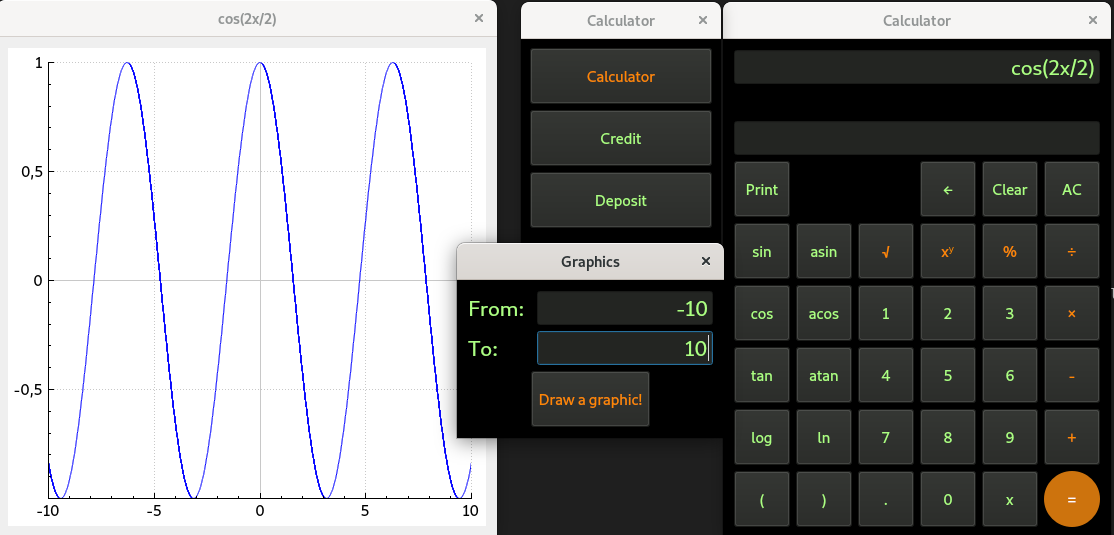
\includegraphics[width=1\textwidth]{images/Main_calculator.png}}
\newpage

{\parskip 10mm The credit calculator shows you monthly payment, overpayment on the credit and total payment.}

\center{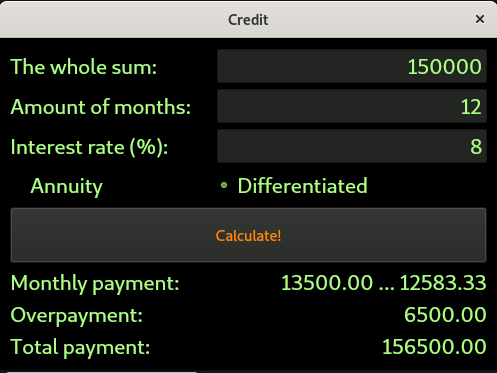
\includegraphics[width=1\textwidth]{images/Credit_calculator.png}}
\newpage

{\parskip 10mm The deposit calculator counts accrued interest, tax amount and the deposit amount by the end of the term.}

\center{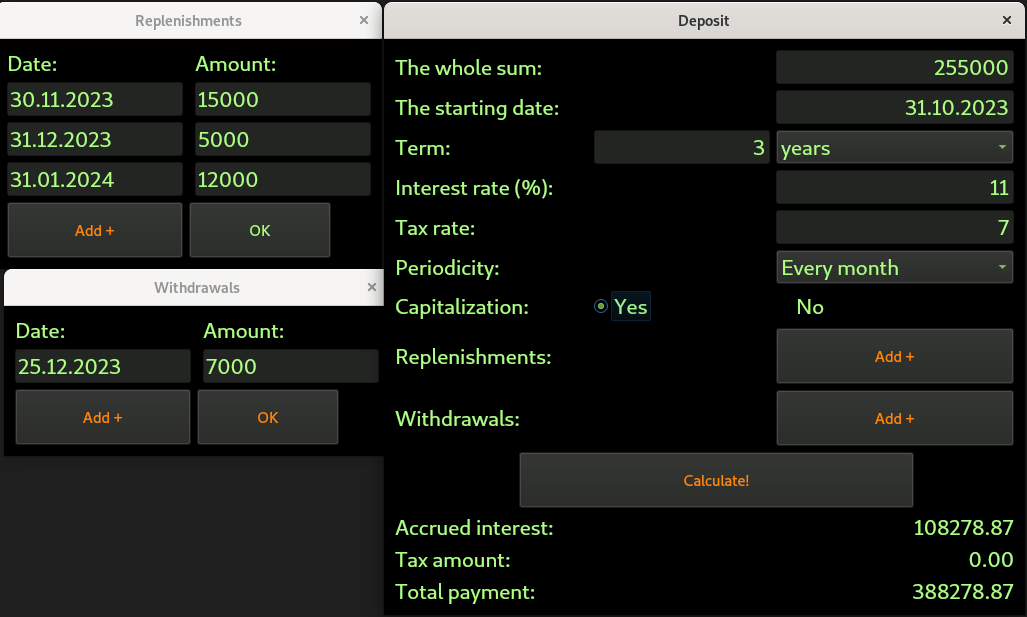
\includegraphics[width=1\textwidth]{images/Deposit_calculator.png}}

\end{abstract}
\tableofcontents
\newpage

\section{Installation}
To install and run this program use the \textit{install} target of the Makefile:
\begin{verbatim}
make install
\end{verbatim}

To uninstall use the \textit{uninstall} target:
\begin{verbatim}
make uninstall
\end{verbatim}

\section{Making an archive}
It is possible to archive the program using the \textit{dist} target of the Makefile:
\begin{verbatim}
make dist
\end{verbatim}

\section{Running tests}
To run style tests use the \textit{style\_check} target:
\begin{verbatim}
make style_check
\end{verbatim}

To run functional tests use the \textit{test} target:
\begin{verbatim}
make test
\end{verbatim}

To check the test coverage use the \textit{gcov\_report} target. It generates an html file containing all the relevant data.
\begin{verbatim}
make gcov_report
\end{verbatim}

To check for the memory leaks use the \textit{leaks} target:
\begin{verbatim}
make leaks
\end{verbatim}

\section{Cleaning}
To clean the directory from all generated files use the \textit{clean} target of the Makefile:
\begin{verbatim}
make clean
\end{verbatim}


\end{document}
